\section{Especificação Arquitetural e Adaptações de Hardware}

A microarquitetura do processador MIPS monociclo implementa o conjunto fundamental de instruções MIPS32 sob modelo Harvard com barramentos independentes para instruções e dados \cite{patterson_mips}.

\subsection{Caminho de Dados Parametrizado (Datapath)}
O caminho de dados no módulo \texttt{datapath.v} possui parametrização integral com \texttt{parameter DATA\_WIDTH = 32} e \texttt{ADDR\_WIDTH = 32} em conformidade com o padrão IEEE 1364-2005 \cite{verilog_std}. Os blocos fundamentais articulam-se da seguinte forma:

\begin{itemize}
    \item Banco de registradores (\texttt{reg\_file.v}): matriz de 32 registradores de 32 bits com duas portas de leitura combinacionais e uma porta de escrita síncrona na borda positiva do clock. O registrador \$0 é fixado em zero;
    \item Unidade lógica e aritmética (\texttt{alu.v}): módulo combinacional que executa operações aritméticas e lógicas. A subtração reaproveita a estrutura do somador computando $A + \overline{B} + 1$, a comparação \texttt{slt} emprega avaliação com sinal via \texttt{\$signed}, e o deslocamento \texttt{sll} opera pelo campo \texttt{shamt} da instrução ($B \ll \text{shamt}$), conforme ilustrado na Fig. \ref{fig:esquematico_alu};
    \item Sinalizador de zero: computado por redução unária rápida $\text{zero} = \sim|\,\text{alu\_result}$, determinando a condição de branch;
    \item Extensor de sinal (\texttt{sign\_extend.v}): converte imediatos de 16 bits para 32 bits replicando o bit mais significativo.
\end{itemize}

\begin{figure}[htbp]
\centering
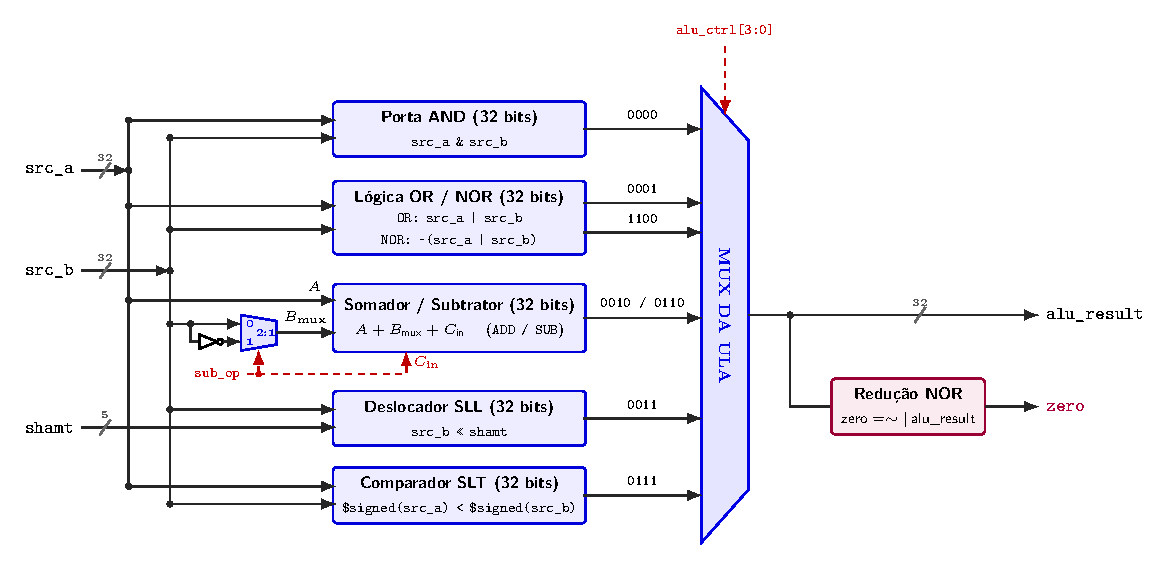
\includegraphics[width=1.00\columnwidth]{000-figuras/esquematico_alu.pdf}
\caption{Esquemático estrutural da Unidade Lógica e Aritmética (ULA) de 32 bits com multiplexação de operações e sinalizador de zero.}
\label{fig:esquematico_alu}
\end{figure}

A restrição temporal da microarquitetura monociclo impõe que o período mínimo de relógio ($T_{\text{clk}}$) acomode a propagação cumulativa da instrução de maior latência, tipicamente a leitura em memória (\texttt{lw}), definida analiticamente por:
\begin{equation}
    T_{\text{clk}} \ge t_{\text{pc}} + t_{\text{rom}} + t_{\text{rf\_read}} + t_{\text{alu}} + t_{\text{ram}} + t_{\text{mux}} + t_{\text{rf\_setup}}
\end{equation}
onde os termos denotam as latências do PC, memórias de instruções e dados, leitura e setup do banco de registradores, ULA e multiplexação. Essa limitação de desempenho justifica diretamente a segmentação em estágios de pipeline no projeto evolutivo do processador.

\subsection{Lógica de Seleção de Próximo PC e Saltos}
No módulo \texttt{datapath.v}, a seleção do endereço da próxima instrução é materializada pela instanciação estrutural dos multiplexadores \texttt{mux\_branch}, \texttt{mux\_jump} e \texttt{mux\_jr} em cascata de prioridade. Esse circuito conecta as saídas intermediárias \texttt{pc\_next\_branch} e \texttt{pc\_next\_jump} até convergir no barramento final \texttt{next\_pc}, conforme esquematizado na Fig. \ref{fig:next_pc}.

\begin{figure}[htbp]
\centering
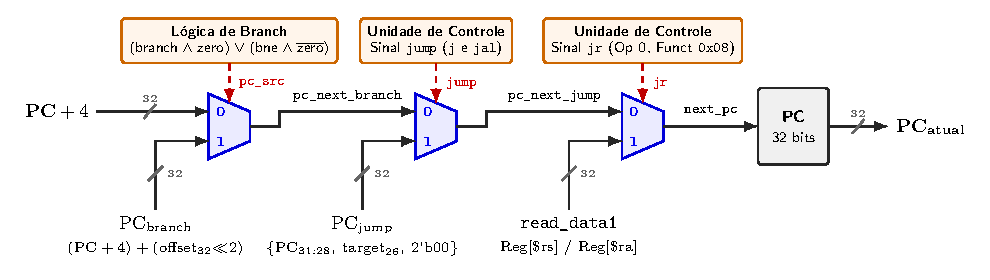
\includegraphics[width=0.92\columnwidth]{000-figuras/esquematico_next_pc.pdf}
\caption{Esquemático da lógica de seleção do próximo PC em cascata no caminho de dados (\texttt{beq}, \texttt{bne}, \texttt{j}, \texttt{jal} e \texttt{jr}).}
\label{fig:next_pc}
\end{figure}

A lógica de decisão obedece à seguinte estrutura hierárquica:
\begin{enumerate}
    \item Desvio condicional com instruções \texttt{beq} e \texttt{bne}:
    \begin{equation}
        \text{pc\_src} = (\text{branch} \land \text{zero}) \lor (\text{bne} \land \overline{\text{zero}})
    \end{equation}
    Seleciona entre $\text{PC}+4$ e o endereço de branch $(\text{PC}+4) + (\text{offset}_{32} \ll 2)$;
    \item Salto incondicional e chamada com link com instruções \texttt{j} e \texttt{jal}: o multiplexador seleciona entre o estágio de branch e o endereço de salto formado por:
    \begin{equation}
        \text{PC}_{\text{jump}} = \{\text{PC}+4[31:28],\; \text{target}[25:0],\; \text{2'b00}\}
    \end{equation}
    Na instrução \texttt{jal}, o endereço de retorno $\text{PC}+4$ é gravado no registrador \$ra via multiplexador com controle $\text{mem\_to\_reg} = \text{2'b10}$ e $\text{reg\_dst} = \text{2'b10}$;
    \item Retorno de função com instrução \texttt{jr}: o multiplexador final seleciona entre o resultado dos estágios anteriores e o dado do registrador \texttt{read\_data1} via sinal \texttt{jr}, garantindo prioridade no fechamento do ciclo.
\end{enumerate}

A unidade de controle possui uma trava de segurança para o sinal de escrita:
\begin{equation}
    \text{reg\_write} = \text{reg\_write\_wire} \land \overline{\text{jr}}
\end{equation}
Essa porta lógica impede que a instrução de retorno sobrescreva o registrador \$ra com dados residuais da ULA.

\subsection{Engenharia de Integração para o Procedimento de Ordenação}
A execução do código de máquina \texttt{sort.bin}, compilado a partir do assembly \texttt{sort.s} com base no procedimento canônico de ordenação de Patterson e Hennessy \cite{patterson_mips}, exigiu soluções dedicadas em nível de hardware para operar sem modificar o binário original.

\subsubsection{Expansão do ISA}
O hardware incorporou suporte nativo a três instruções requeridas pelo algoritmo:
\begin{itemize}
    \item Instrução \texttt{sll}: o barramento do campo \texttt{instr[10:6]} foi conectado diretamente à porta \texttt{shamt} da ULA;
    \item Instrução \texttt{slti}: o opcode \texttt{001010} foi mapeado na controladora principal para forçar a operação \texttt{slt} da ULA sobre o operando imediato estendido;
    \item Instrução \texttt{bne}: o opcode \texttt{000101} foi integrado à lógica combinacional de desvio.
\end{itemize}

\subsubsection{Bypass de Endereçamento do MARS}
O montador MARS \cite{mars_simulator} aloca o segmento de código a partir do endereço virtual \texttt{0x00400000}. Para evitar violação de barramento na memória física local de 256 palavras, implementou-se uma máscara na ROM:
\begin{lstlisting}[style=estiloVerilog]
assign instr = rom[addr[9:2]]; // Indexa palavras locais
\end{lstlisting}
Esta máscara ignora os 22 bits mais significativos, viabilizando o mapeamento direto das instruções do simulador para a memória estática em silício.

\subsubsection{Bootloader de Hardware no Reset}
O procedimento \texttt{sort} pressupõe pilha inicializada e argumentos nos registradores \texttt{\$a0} e \texttt{\$a1}. O registrador de reset do banco de registradores atribui:
\begin{equation}
    \text{sp} \leftarrow 256, \quad \text{a0} \leftarrow 0, \quad \text{a1} \leftarrow 5
\end{equation}
Essa inicialização posiciona o topo da pilha no limite da memória RAM e direciona o vetor para a base da memória de dados.
